\subsection{M.PC.12 - Efficienza delle contromisure nei rischi}
\begin{figure}[H]
    \centering
    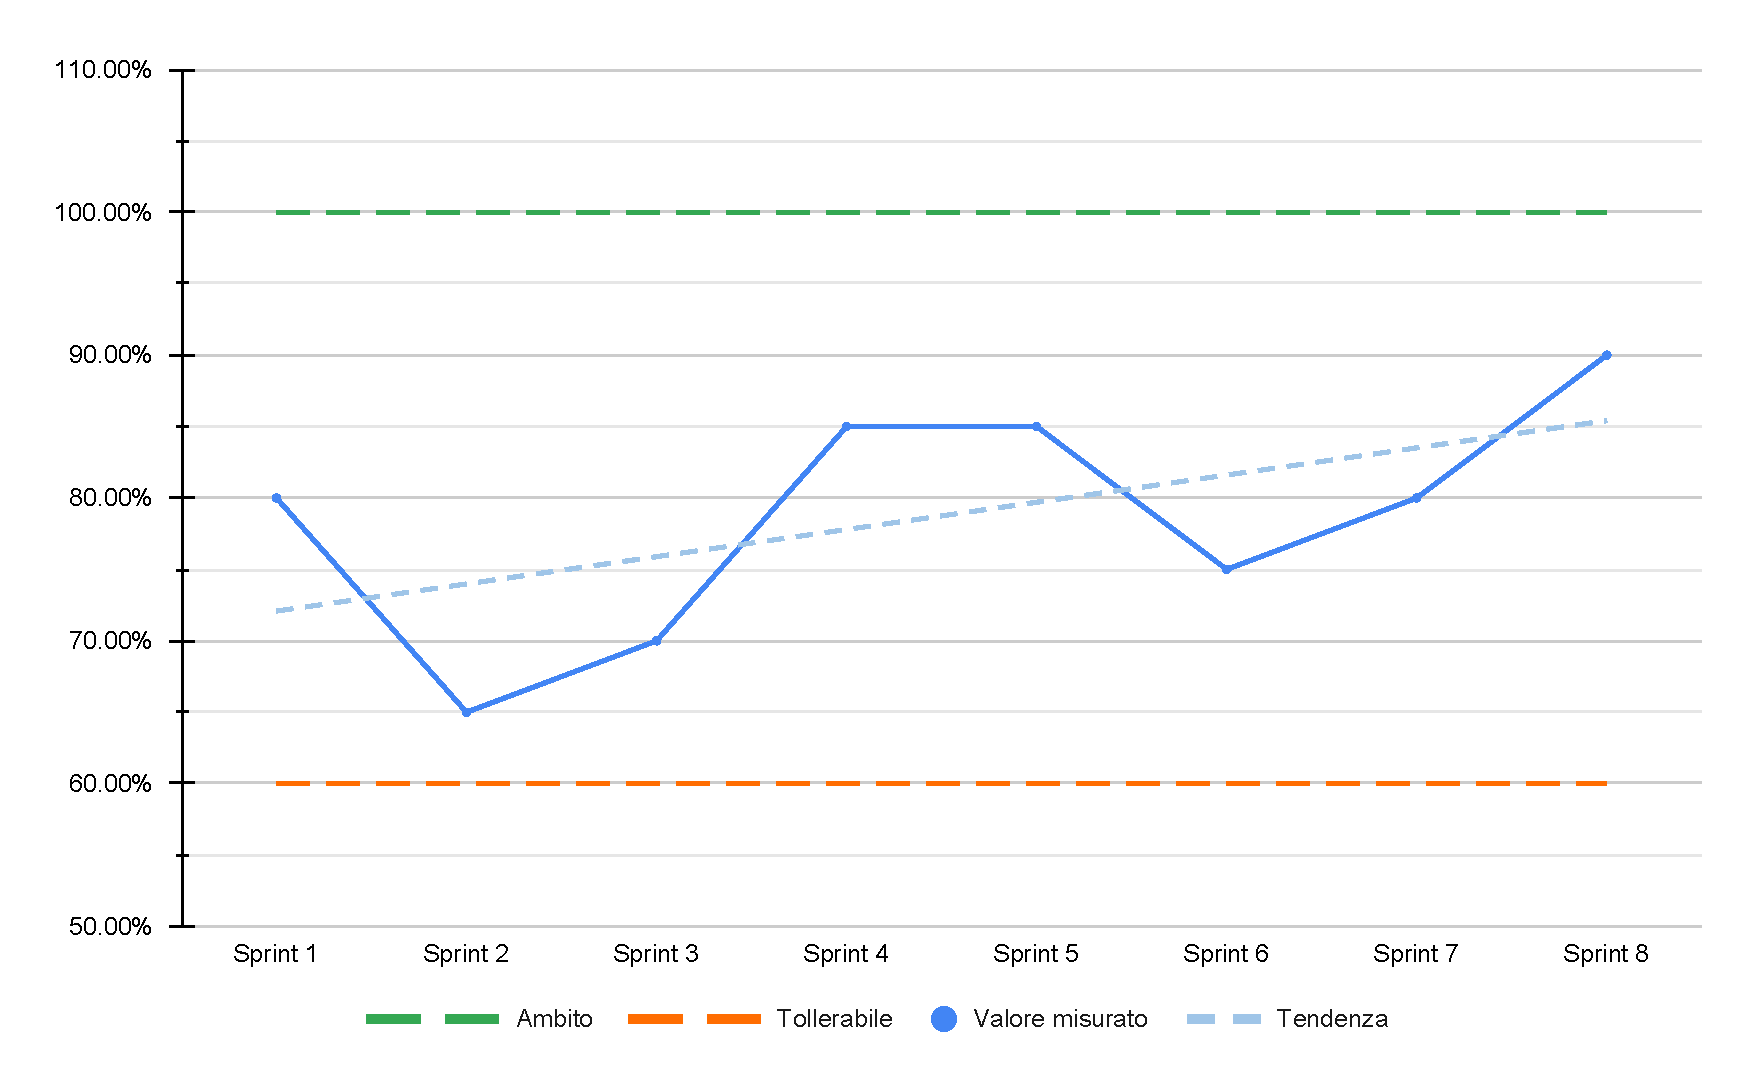
\includegraphics[width=\textwidth]{assets/efficienza_contromisure.pdf}
    \caption{M.PC.12 - Efficienza delle contromisure nei rischi}
\end{figure}

\par L'andamento dell'efficienza delle contromisure nei rischi in via di miglioramento descrive un percorso evolutivo da una fase iniziale di adattamento e apprendimento a una successiva fase di miglioramento e ottimizzazione continua. Inizialmente, le contromisure non raggiungevano il livello desiderato di efficacia, mostrando una necessità di aggiustamenti e raffinamenti. Questa fase è caratterizzata da una curva di progresso inizialmente stabile, mentre il team sperimentava con nuove strategie o affronta le prime difficoltà operative.
Con il passare del tempo e l'accumulo di esperienza, l'andamento dell'efficienza delle contromisure mostra segni di miglioramento. Questo progresso è alimentato dall'implementazione di feedback provenienti dall'esperienza pratica, dall'adozione di migliori pratiche, o dall'introduzione di tecnologie che aumentano la capacità del team di rispondere in modo rapido ed efficace ai rischi identificati.
L'andamento in via di miglioramento rappresenta un ciclo di adattamento e perfezionamento continuo. Testimoniando la capacità del team di affrontare le sfide con strategie sempre più efficaci e mirate nel tempo. Questo non solo riduce l'impatto dei rischi identificati, ma rafforza anche la capacità dell'organizzazione di gestire in modo proattivo e resiliente le incertezze e le variazioni ambientali.
